
\begin{figure}[h!]
\centering
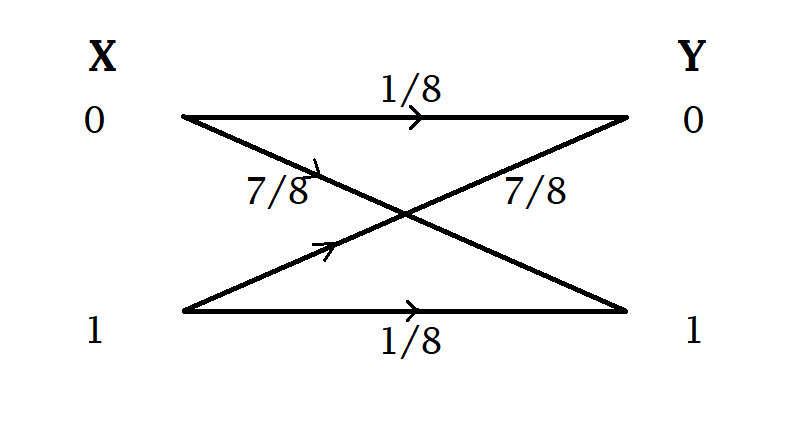
\includegraphics[width=\columnwidth]{solutions/24/Figure.png}
\caption{Binary symmetric channel}
\label{fig:BSC}
\end{figure}

Let random variables, $X \in \{0,1\}$ denote the bit transmitted and $Y \in \{0,1\}$ denote the output bit received.
\\From the given information, 
\begin{align}
    \pr{X=0} = \frac{9}{10}\\
    \pr{X=1} = 1-\pr{X=0} = \frac{1}{10}
\end{align}
Also given, transition probability = $\frac{1}{8}$. Transition probability is the probability with which the bit is transmitted correctly. That gives, 
\begin{align}
    \pr{Y=1|X=1}=\pr{Y=0|X=0}=\frac{1}{8}
\end{align}
\begin{multline}
\text{Probability that the bit is not transmitted correctly}  \\
= 1-\text{transition probability}\\
= 1-\frac{1}{8} = \frac{7}{8}
\end{multline}
That gives,
\begin{align}
    \pr{Y=0|X=1}=\pr{Y=1|X=0}=\frac{7}{8}
\end{align}
Let E denote the event that bit is transmitted incorrectly. Probability of error, $\pr{E}$
\begin{multline}
    \pr{E} = \pr{X=0}\pr{Y=1|X=0}\\ + \pr{X=1}\pr{Y=0|X=1}
\end{multline}
On substituting the values,
\begin{align}
    \pr{E} & = \frac{9}{10}\times\frac{7}{8} + \frac{1}{10}\times\frac{7}{8} \\
    & = \frac{63}{80} + \frac{7}{80}\\
    & = \frac{7}{8}
\end{align}
\rightline{Answer: No option matches}


